\chapter{Plantejament de l'hipòtesi}

Al ser l'implementació de les funcions no-lineal un assumpte lleugerament conflictiu entre els diversos models de xarxes neuronals quàntiques havia decidit des de un principi centrar-me en aquest assumpte en concret. Podria haver anat per al altres vies com la generació d'imatges amb color o l'implementació d'un d'una porta $X$ en una part especifica del circuit quàntic que genera les imatges, que al posar-la o no, el model generes dos tipus d'imatge a través del mateix circuit. Tanmateix, les dues propostes requerien de desenvolupar nous conceptes, llavors al no tindre el coneixements necessaris per poder desenvolupar-les vaig descartar aquestes opcions. 

La pregunta a investigar és la següent: \\
L'incorporació d'una funció no-lineal en el circuit quàntic del model, a partir d'una mesura parcial, causa que el model arribi més ràpidament al punt òptim?

En altres paraules, volia veure si la mesura parcial repercutia positivament en la eficiència del model, fent que la generació de les imatges desitjades es dones a terme en un menor temps. 

Sembla una qüestió senzilla, però la dificultat del experiment radica en crear la xarxa neuronal en si, amb totes les seves parts accessibles per poder fer els canvis que siguin necessaris. L'única manera de fer-ho seria programant el model. 

\chapter{Programació del model}

Posteriorment a començar a programar el model, jo ja sabia que ho havia de realitzar en Python, ja creat petits algoritmes abans de començar aquest treball i tenia experiència construint i executant circuits quàntics amb Cirq, una eina desenvolupada per Google. A més a més, sabia de l'existència de TensorFlow Quantum \cite{tfq}, una altra eina desenvolupada per Google destinada a la creació de xarxes neuronals quàntiques i algoritmes de \textit{quantum mechine learning} en general. També tenia experiència en aquest \textit{framework}. Llavors TensorFlow Quantum va ser la meva primera opció, tenia pensat basar el meu codi en el tutorial de TensorFlow sobre un xarxa convolucional generativa adverbial. Havia de canviar el generador per un circuit quàntic que s'obtimitza a partir d'un diferenciador automàtic provinent de TensorFlow Quantum. Els canvis que corresponien al discriminador simplement havien de ser un canvi d'arquitectura, passar d'una xarxa més complexa a una de més simple que només consistia en unes poques capes totalment connectades. 

El primer problema que em vaig trobar va ser la creació del \textit{data set} que alimentar a la xarxa discriminativa. A causa de la peculiaritat de les imatges que volia generar\footnote{Usualment les imatges que componen els \textit{datasets} utilitzats en \textit{deep machine learning} són extretes de bancs d'informació amb mides enormes. En el meu cas, havien de ser generades per mi, per tant havia de convertir matrius de Numpy en \textit{datasets} per TensorFlow.}. Recordo que en va costar arribar a tindre la solució a aquest problema. 

\section{Discriminador}

Una vegada ja tenia fet el \textit{dataset} em vaig posar a fer el model. En el tutorial per una \href{https://www.tensorflow.org/tutorials/generative/dcgan}{DCGAN (GAN conolucional)} els dos models eren entrenats per la funció \code{train\_step}. En aquesta es crida a la funció \code{tf.GradientTape} per guardar el diferenciador automàtic. El problema que vaig dintre amb aquesta funció es que directament no funcionava amb el discriminador, aquest no era optimitzat. Després de intentar solucionar l'error pels meus propis medis, mirant la causa d'aquest i de buscar a forums la solució o causa, em vaig rendir. Ja havia estat uns quants mesos intentant desenvolupant el model amb TensorFlow i TensorFlow Quantum. Havia creat les capes del generador quàntic manualment, també ho havia fet amb el optimitzador. Tenia el model gairebé acabat, però al no poder optimitzar el discriminador em vaig veure obligat a canviar d'estrateiga. 

Existeixen dos grans \textit{frameworks} per crear i executar circuits quàntics: Cirq \cite{cirq}, desenvolupat per Google i Qiskit \cite{qiskit}, creat per IBM. Una vegada vaig decidir no continuar amb Cirq, havia de provar amb Qiskit. La veritat, havia d'haber començar amb Qiskit des de el principi, és més útil (té moltes més característiques), i el més important, té una gran comunitat, per tant, es més fàcil trobar solucions als error que pots tenir i és més fàcil trobar a persones disposades a ajudar-te.

Al igual que Cirq té un \textit{framework} per poder desenvolupar xarxes neuronals, TensorFlow Quantum, Qiskit també té el seu PyTorch \cite{pytorch_2019}, no obstant no té una integració tan directa, ja que no estan desenvolupats per el mateix equip, ni la mateixa companyia. 

Per tant, al canviar de Cirq a Qiskit, també havia de canviar de TensorFlow a PyTorch, no obstant, no tenia res d'experiencia amb PyTorch, sabia que seria més complicat, i tenia raó. No vaig ni aconseguir crear el \textit{dataset} que contenia les imatges que alimentar al discriminador. 

Després d'intetar-lo amb TensorFlow Quantum i amb PyTorch, vaig decidir prescindir de \textit{frameworks} per crear models de \textit{machine learning}, el discriminador, al ser una xarxa tan simple, la podia crear des de zero. Llavors vaig començar a buscar codi, d'una xarxa neuronal que havia estat feta amb Numpy, una llibreria de Python per fer càlculs amb vectors i matrius que havia fer servir des de que vaig començar amb Python.

Després de provar dues opcions que més o menys m'agradaven\footnote{Busca codi estructurat d'una forma en concret, que estigui dissenyat amb \textit{Object Oriented Programming}, una forma d'escriure codi en el qual tot s'implementa en un objecte.}, va aparèixer un repositori\footnote{\href{https://github.com/mnielsen/neural-networks-and-deep-learning}{link del respositori}} de Michael Nielsen, un dels autors de \textit{Quantum Computation and Quantum Information} \cite{QCandQI} que em va salvar. 

El repositori tenia codi que estava estructurat d'una forma que m'agradaba i encara més important, que l'entenia. Inclús tènia diverses versions d'una xarxa neuronal, amb un nivell de complexitat diferent. Llavors, a partir del model més simple que havia en el repositori, veure el codi original al apèndix \ref{lst:disc_original}, vaig començar a desenvolupar el discriminador. 

Com es pot veure al codi final per el discriminador, he fet bastants canvis, però ho he canviat l'estructura o el funcionament teòric, la majoria són per tindre més funcionalitat, com per exemple l'enmagatzematge de les dades per poder al final veure-les en gràfic. Però el canvi més important és que inclou les dues formes d'optimitzar el model, amb dues funcions de pèrdua que funcionen de manera diferents però que són el mateix, la \textit{Binary Cross Entropy} i la \textit{MinMax}. Ja he parlat d'aquestes dues funcions en la part teòrica del treball, però a mode de recordatori, amb la primera s'agafa una imatge falsa o una real, i s'altera la funció, mentre que amb la \textit{MinMax} depenent de si es una imatge falsa o una real, s'utilitza una funció diferent. Això en el codi està materialitzat en dues funcions\footnote{Funcions de Python.} diferents, \code{backprop\_bce()} i \code{backprop\_minimax()}. No fa falta entrar en detall sobre que va cadascuna de les funcions, degut a que, fan el mateix i no tenen ninguna diferencia en termes de eficàcia o rapidesa. Les vaig fer tan sols per comprovar que no hi hauria ninguna diferencia. El codi final del discriminadors es pot veure al apèndix \ref{lst:disc_final}. També en el repositori del treball hi ha un altre arxiu anomenat \code{discriminator.py}, que conté una altre versió en la qual intentava implementar diverses funcions d'activació en el model, però no ho vaig aconseguir, tanmateix, no em preocupa perquè no es una part vital del treball, no passa res per tindre el discriminador només amb la sigmoide. 

\section{Generador}

El desenvolupament de l'altre part del model, el generador, va ser molt diferent. Després de provar a fer-ho amb TensorFlow, sense resultats, no tenia altra opció que fer-ho tot manualment i jo mateix\footnote{No em vaig ni plantejar buscar codi per internet perquè pensava que els autors dels paper que vaig llegir, les úniques persones que sabia que podien tindre el codi, no el penjarien.}, no obstant, ja tenia experiència en fer pseudo-xarxes neuronals quàntiques. Sabia perfectament el que tenia que fer, i com ho havia de fer. Implementar el mètode de \textit{parameter shift} en els circuits quàntics de l'article en el que vaig basar el treball \cite{QGAN_exp}. 

Una vegada vaig crear els circuits quàntics amb una funció fins a un punt en el qual sentia que ja estava tot perfecte, em vaig posar amb la optimització. 

Penso que és més fàcil de fer que el \textit{backpropagation} en una xarxa neuronal clàssica. 
Primer de tot cal remarcar que el model s'optimitza a partir d'un \textit{batch}, es a dir, un grup d'imatges, en aquest cas, un grup de dades, extretes del \textit{latent space}. Per tant, s'agafa la mitjana del errors de cada input, i s'actualizen els paràmetres a partir d'aquesta mitjana. No es mira l'error d'un sol input per optimitzar, s'ha de mirar el de uns quants, s'aquesta manera, l'optimtizació és més robusta. 

El procediment és el següent, s'ha d'agafar els paràmetres a optimitzar, que estaran en la forma d'un vector, escollir un dels paràmetres, i crear el vector de pertubació. Es a dir un vector de la mateixa mida que el vector amb els paràmetres, però amb tot de zeros, menys a la posició del paràmetres que es vol optimitzar. 

Llavors es creen dos vectors de paràmetres nous multiplicant $\pm\frac{\pi}{4}$ pel vector de pertubació, i sumant el resultat al vector de paràmetres original. A continuació, es creen dues imatges, cadascuna per a cada grup de paràmetres, una amb el terme $\pm\frac{\pi}{4}$ positiu i l'altra amb el negatiu. Per últim, es mira la funció de pèrdua per a cada imatge generada i es treu la diferencia entre elles. El resultat es sumat a un vector que té la mateixa mida que el vector de paràmetres. Al començament de l'iteració, aquest vector és zero, però segons es va optimitzat s'ha li van sumant els errors. Això es fa per a cada paràmetre del circuit per un input, i per a cada input dintre del \textit{batch} a optimitzar.
\begin{figure}
	\label{fig:alg_gen}
	\HRule \\[-.5cm]
	\begin{algorithmic}[1]
		\State{$\nabla = 0$} \Comment{Creació del vector  $\nabla$ que te la mateixa mida que $\theta$}
		\For{soroll en batch}
		\For{paràmetre $\theta_i$ en  $\theta$}
		\State{$\Delta_i = 0$} \Comment{Creació del vector pertubació d'acord amb el vector $\theta_i$}
		\State{$\theta^{+}_i = \theta + \frac{\pi}{4}\Delta_i$}
		\State{$\theta^{-}_i = \theta - \frac{\pi}{4}\Delta_i$}
		\\
		\State{Imatge\textsubscript{1} = generador(soroll, $\theta^+_i$) } 
		\State{Imatge\textsubscript{2} = generador(soroll, $\theta^-_i$) } \Comment{Generació de les imatges}
		\\
		\State{Predicció\textsubscript{1} = discriminador(Imatge\textsubscript{1})} 	\State{Predicció\textsubscript{2} = discriminador(Imatge\textsubscript{2})} \Comment{El discriminador posa una etiqueta a cada imatge}
		\\
		\State{Diferencia\textsubscript{$i$} = $\mathcal{L}$(Predicció\textsubscript{1}) - $\mathcal{L}$(Predicció\textsubscript{2})}
		\\
		\State{$\nabla_\theta = \nabla_i + $ Diferencia\textsubscript{$i$}} \Comment{On $\mathcal{L}$ és la funció de pèrdua del generador}
		\EndFor
		\EndFor
		\\
		\For{$\theta_i$ en $\theta$ i $\nabla_i$ en $\nabla_\theta$} \Comment{Per a cada paràmetre i per a cada error}
		\State{$\theta^{t+1}_i = \theta_i + \frac{\eta}{M}\nabla_i$} \Comment{Actualització del paràmetre amb la mitjana de l'error que correspon a aquest paràmetre}
		\EndFor
	\end{algorithmic}
	\HRule \\[-.4cm]
	\caption{\textbf{Pseudocodi per una xarxa generativa adversativa.} Em refereixo al input de la xarxa generacional com a soroll, ja que és més acertat d'aquesta manera. El vector $\nabla$ té la mateixa mida que el vector de paràmetres $\theta$, cal notar que també té la mateixa mida els vectors $\theta^\pm_i$, degut a que aquests vectors són $\theta$ per amb una alteració al paràmetre $\theta_i$. Les paraules \textit{generador} i \textit{discriminador} denoten els respectius models, per tant, \textit{Imatge\textsubscript{$i$}} i \textit{Predicció\textsubscript{$i$}} són els outputs del models.}
\end{figure}

Quan ja s'han calculat tot els errors, s'agafa el vector que els conte que és multiplica pel \textit{learning rate}, i es divideix per el nombre d'imatge del \textit{batch}, d'aquesta manera fent la mitjana aritmètica del errors. El resultat es suma als paràmetres originals, d'aquesta manera completant una iteració. 

El pseudocodi per aquest procediment es pot trobar en la figura \ref{fig:alg_gen}. 
 
En la figura es pot veure que es crida al discriminador perquè posi etiquetes a les dues imatges generades, això es per poder avaluar aquestes etiquetes amb la funció de pèrdua, per després poder agafar la diferencia i d'aquesta manera calcular el gradient. La funció de pèrdua és la part que correspon al generador, ja que la etiqueta que han de tenir aquestes imatges es 1, degut a que es vol que siguin com les imatges reals. El codi per el generador es pot trobar en l'apèndix, \ref{lst:gen_final}.

\section{Creació del model}

Quan ja es tenen les dues parts del model, s'ha d'ajuntar d'alguna manera. El que jo he fet es posar-lot tot en una classe de Python anomenada \code{Quantum\_GAN}, que conté les funcions per definir el model, executar-lo, guardar les seves dades i per crear els gràfics que serveixen per avaluar l'eficiència del model. No fa falta entrar en detall, sobre aquesta part particular del codi. Només cal mencionar que és el tros de codi que junta tot, tant el discriminador i el generador, coma altres funcions que són necessàries, com per exemple la sigmoide. Aquestes funcions que no estan tant en l'arxiu del generador com el discriminador es troben en \code{functions.py}. 

Tanmateix s'han de tenir en compte algunes de les funcionalitats d'aquesta classe, com la creació de les gràfiques i com circulen les dades del generador al discriminadors. D'aquesta última qüestió parlaré a continuació. 

A la funció de la classe \code{Quantum\_GAN} que s'utlitza per entrenar, \code{Quantum\_GAN.train()} se li dona, entre altres inputs, un dataset amb imatges reals i el soroll que forma part del espai latent per poder entrenar el generador. Aquest dataset el divideix en grups d'imatges (els batch), cada batch conté tant imatges reals, com soroll en la mateixa quantitat.

En una iteració primer s'optimitza el generador, que substitueix el soroll del batch amb les imatges que genera. Llavors es passa el batch al discriminador que s'optimitza tant amb les imatges reals com amb les imatges falses. Aquest és el procés per el qual s'optimitzen els dos model. No obstant, aquesta funció dona a terme altres coses que són necessàries per la creació dels gràfics, per exemple, selecciona una imatge real aleatòria i una de falsa per avaluar la funció de pèrdua en l'iteració, també les etiquetes utilitzades en l'avaluació, s'utilitzen per la creació d'un gràfic que mostra l'evolució dels valors de les etiquetes a través de tota l'optimització. 

\section{Execució del model}

No obstant en l'arxiu \code{qgan.py}, no es troba l'execució del model, només està la definició de la classe \code{Quantum\_GAN}. Això és perquè el codi realment s'executa en l'arxiu \code{main.py}\footnote{Veure apèndix \ref{lst:main}}. Aquest és l'únic arxiu que té codi que realment s'executa, els altres arxius només tenen definicions. Per projectes relativament grans, com aquest, convé tenir un arxiu que fa tot el treball, el qual crida a totes les funcions definides en altres arxius i les executa d'una manera ordenada. 

Com es pot veure en l'apèndix, \ref{lst:main}, aquesta arxiu té molt poc codi. En ell només es crea amb Numpy el dataset, es defineix el discriminar i el generadors, es crea el model amb \code{Quantum\_GAN}, i es crida la funció \code{Quantum\_GAN.train()} per optimitzar-lo. Al acabar l'optimització es criden les funcions \code{Quantum\_GAN.plot()}, \code{Quantum\_GAN.create\_gif()} i \code{Quantum\_GAN.save()}, les quals donen a terme funcions complementàries com la creació de les gràfiques, la creació d'un GIF que mostra com les imatges vam evolucionant al llarg de l'optimització, i l'emmagatzematge de les dades rellevant que s'han creat durant l'optimització.  

Les imatges que vaig escollir per generar són les mateixes que van generar en l'article en el que em vaig basar. No entraré molt en detall sobre les distribucions concretes que formen les imatges, però per tindre una imatge general sobre com són, es pot veure la figura, \todo{poner la figura donde se ven como 4 imagenes o algo asi no se ya lo veras en un futuro depende de como queden}.

Si executen el model, amb un mida de batch de $10$, tant el \textit{learning rate} del discriminador com del generador a $0.1$, i un total de iteracions de $400$, hi ha una garantia d'arribar a la convergència desitjada, es dir que, que els dos models arriben al equilibri de Nash i no poden continuar l'optimització. En aquest punt és quan les imatges falses i les reals són iguals.

\begin{figure}
	\label{fig:comp_imatge}
	\begin{subfigure}{0.51\textwidth}
		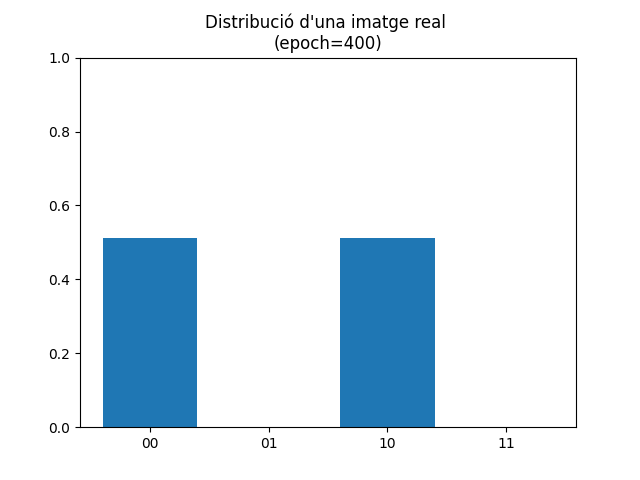
\includegraphics[width=\linewidth]{figures/model/real_distribution.png}
		\caption{Distribució d'una imatge real} \label{fig:1a}
	\end{subfigure}%
	\hspace*{\fill}   % maximize separation between the subfigures
	\begin{subfigure}{0.51\textwidth}
		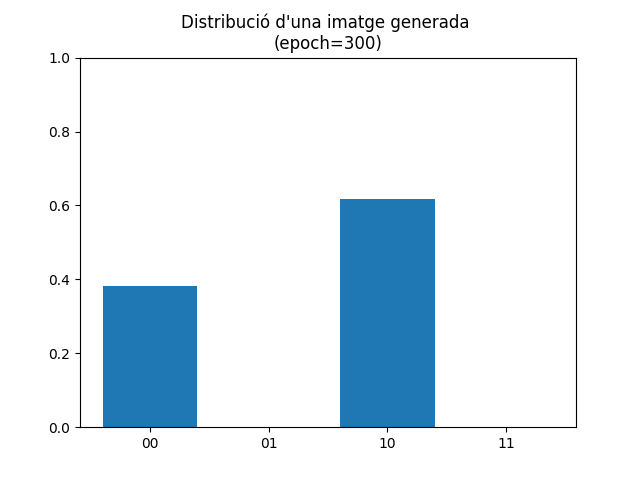
\includegraphics[width=\linewidth]{figures/model/fake_distribution.png}
		\caption{Distribució d'una imatge generada} \label{fig:1b}
	\end{subfigure}%
	\hspace*{\fill}
	\caption{Comparació d'una imatge generada i una real, quan el model ha assolit la convergència. En el eix Y es pot veure el valor d'un píxel, mentre que en l'eix X estan els píxels. }   % maximizeseparation between the subfigures
\end{figure}
\begin{figure}
	\label{fig:labels_loss_400}
	\begin{subfigure}{0.45\textwidth}
		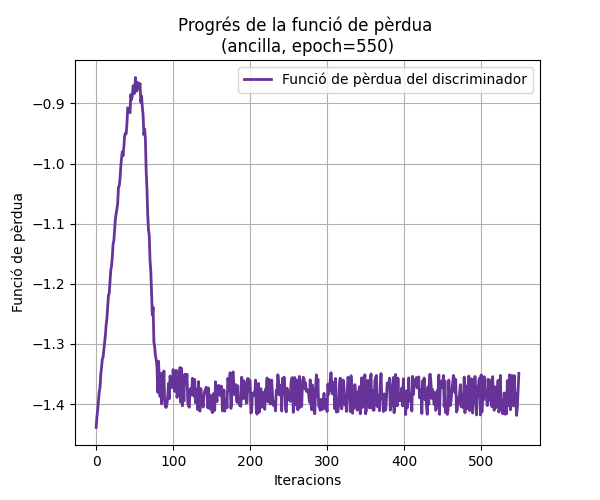
\includegraphics[width=\linewidth]{figures/model/loss_plot.png}
		\caption{Funció de pèrdua per cada iteració. A partir de l'iteració 175, es pot veure com el valor de la funció s'estabilitza en l'interval $(-1.35, -1.4)$, això concorda amb els valors de les etiquetes en les mateixes iteracions, ja que $\log(\frac{1}{2}) + \log(1-\frac{1}{2}) \simeq -1.38$.}\label{fig:loss_400}
	\end{subfigure}%
	\hspace*{\fill}   % maximize separation between the subfigures
	\begin{subfigure}{0.45\textwidth}
		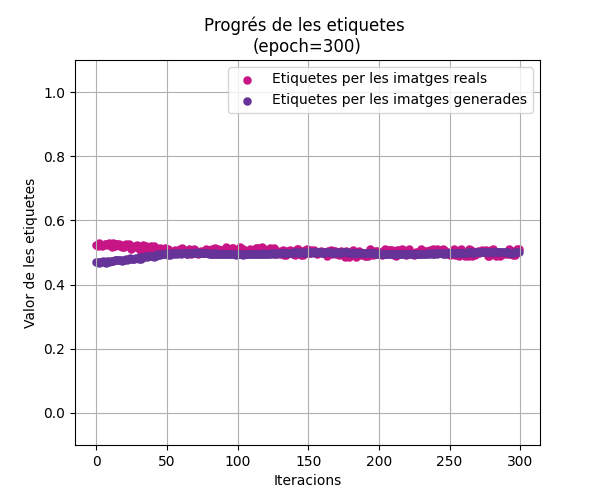
\includegraphics[width=\linewidth]{figures/model/labels_plot.png}
		\caption{Etiquetes per les imatges reals i generades per cada iteració. Es pot observar que els valors de les etiquetes per les imatges reals són més inestables que els valors de les generades. Això es perquè les imatges reals tenen una major variació en els valors dels píxels, mentre que en les generades aquest fet no es tan notable. Per tant el discriminador assigna etiquetes amb una major variació.} \label{fig:labels_400}
	\end{subfigure}%
	\hspace*{\fill}
	\caption{En pot veure com per l'iteració 250, el model ja s'ha estabilitzat, ja que les etiquetes i el valor de la funció de pèrdua convergeixen en un valor.}% maximizeseparation between the subfigures
\end{figure}

En la figura, \ref{fig:labels_400}, es pot veure com les etiquetes pels dos tipus d'imatges van oscil·lant fins a estabilitzar-se. El mateix es pot dir per la funció de pèrdua \ref{fig:loss_400}.  

Degut a que aquests gràfics són molt semblants als seus anàlegs de les GANs clàssiques i que les distribucions reals i generades són pràcticament iguals, com es pot veure a la figura \ref{fig:comp_imatge}. Considero que el model funciona correctament. 



Abans he especificat que al cap de $400$ iteracions podem tenir la garantir d'arribar al punt d'equilibri, no obstant, es pot arribar a aquest punt amb menys iteracions, el que vull dir es que amb $400$ de segur que s'arriva. Això és perquè, com a tots els model de \textit{machine learning} hi ha una part de sort implicada, si els paràmetres inicials són més semblants als paràmetres desitjats, el model assoli-ra la convergència més ràpidament. Per més detalls l'execució del model es pot veure l'apèndix XXX. Tanmateix, per més informació sobre la part experimental del treball es pot veure en l'apèndix XXX.1, en aquest capítol he omitit coses interessants com el meu intent de generació d'imatges a color. 
 
\chapter{Realització del experiment} 

Una vegada havia confirmat el correcte funcionament del model, vaig alterar el generador per poder acomodar els dos tipus de circuits quàntics que necessitava, uns amb un sistema ancilla, i uns altres sense.

Un sistema ancilla, són un grup de qubits sobre els quals es donen a terme operacions però que no es mesuren per treure el output del circuit. Aquests qubits es pot veure molt clar en la figura, \todo{poner figura}. 

Primer de tot he de mencionar que havia de fer alguns canvis al generador per acomodar aquests qubits ancilla. 

Segon, cal notar que no he seguit exactament els mateixos passos que en l'article original. En ell tenen aquesta equació \cite{QGAN_exp}: 
\begin{equation*}
\rho = \frac{\tr_A(\Pi_A \ket{\psi}\bra{\psi})}{\tr(\Pi_A\otimes I_{2^N-2^{N_A}}\ket{\psi}\bra{\psi})}
\end{equation*}

Com ja he comentat en la secció \ref{par_measurament}, no veig com aquesta equació pot tenir sentit, per tant la vaig ometre del meu experiment. 

L'alternativa que he fet servir són els mesuraments de Qiskit, al definir el circuit especifico quins són els qubits que vull mesurar, que són els qubits que formen part del sistema ancilla. No obstant, no sé exactament que és lo que fa Qiskit amb el mesurament. Però si empro aquest procediment en altres circuits, quals sé com han de funcionar, aquest mètode fa el que m'espero\footnote{Parlo del parells de Bell, els circuits quàntics amb entrellaçament més simples que es poden fer.}. 

L'arxiu que utilitzo per fer els experiments és \code{experiment.py}. En ell es pot veure com defineixo dos discriminadors\footnote{Que són iguals en característiques} i dos generadors, que es diferencien per els circuits que utilitzen, un amb qubits ancilla i l'altre sense. Aquests model s'agrupen en parelles per definir dos qGANs. 

Cal notar que els generadors i els discriminadors\footnote{Al principi pensava no tenir els mateixos paràmetres inicials pels discriminadors, però al veure les gràfiques de les etiquetes, l'efecte que tenen aquests és molt notable. Es pot veure com a vegades les etiquetes comencen en uns valors de $1$ i en altres de $0$. \href{https://drive.google.com/file/d/1kYZ1vmNYU17sofNluXFYnoATLfY5B0jG/view?usp=sharing}{link per veure una imatge amb totes les gràfiques} (perdó per l'informalitat)} comencen amb els mateixos paràmetres, per tant en exactament les mateixes condicions, menys els circuits quàntics es clar. També s'utilitza el mateix dataset i altres hiperparàmetres. 

\section{Anàlisi dels resultats}


 